\subsubsection{Macro-caso d'uso - Condivisione}
\paragraph{Diagramma UML}

\begin{figure}[H]
    \centering
    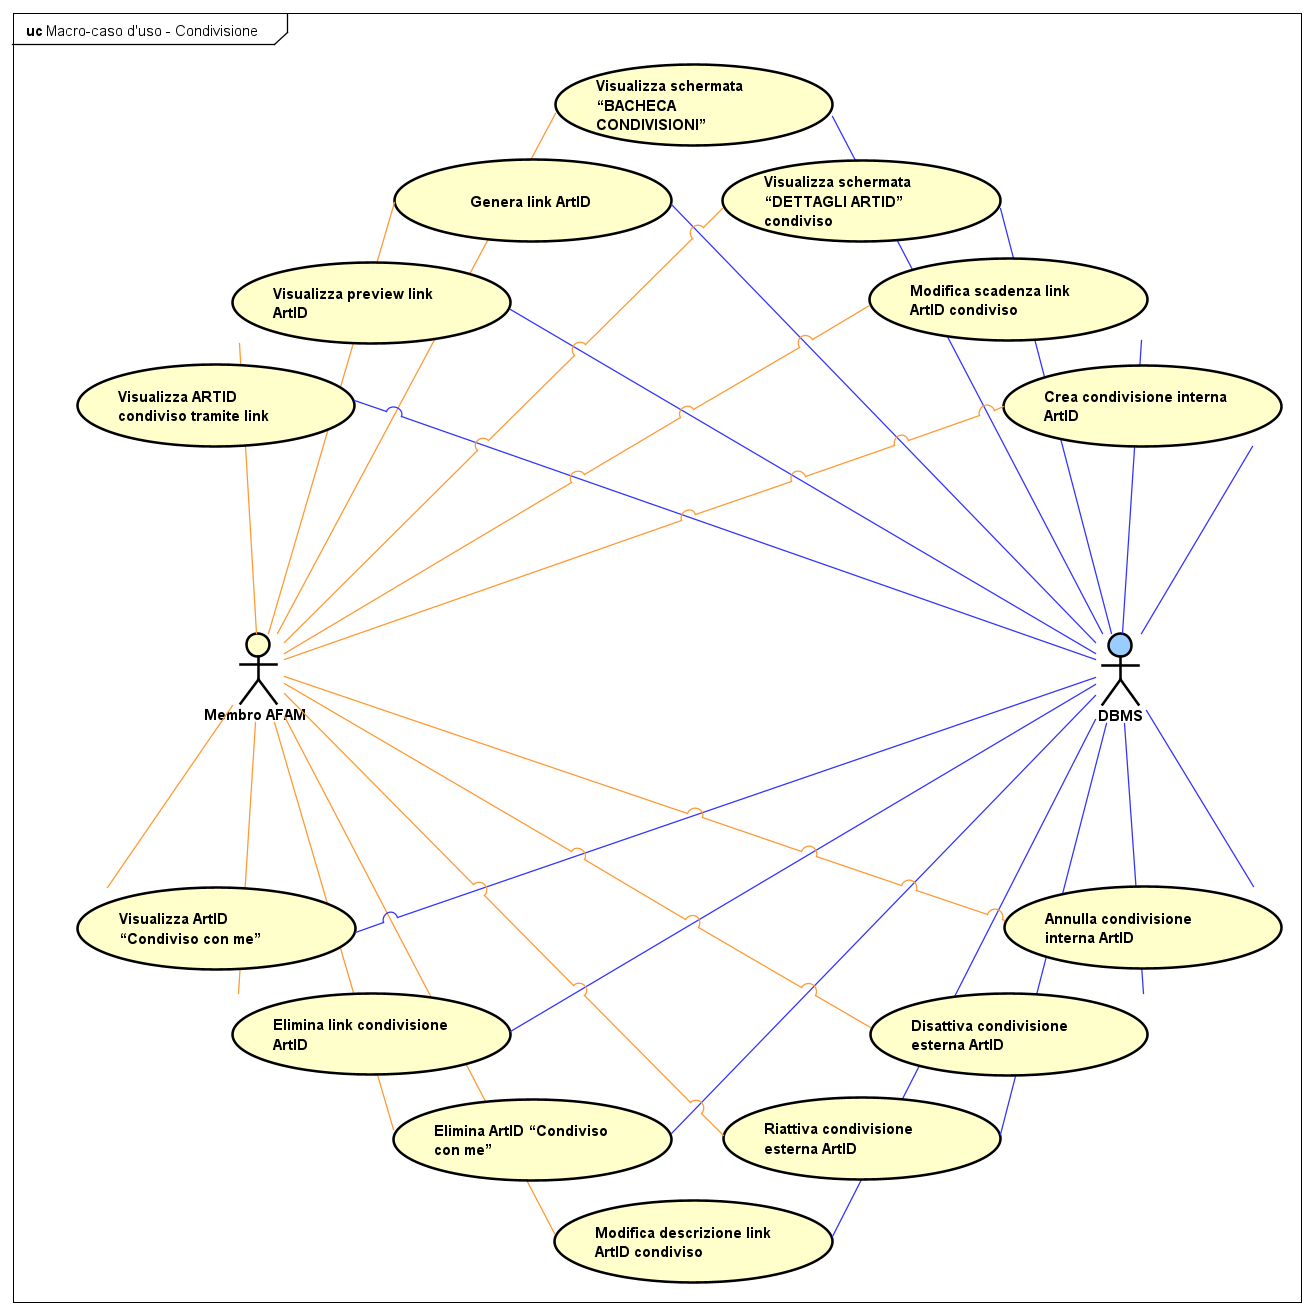
\includegraphics[width=0.95\textwidth, height=0.95\textheight, keepaspectratio]{Immagini/Use-case diagrams/Macro-caso d'uso - Condivisione.png}
\end{figure}

\clearpage

\paragraph{Visualizza ArtID condiviso tramite link}
\par{\noindent Il seguente caso d'uso permette la visualizzazione di un ArtID associato a un link di condivisione e di notificare l'autore dell'ArtID dell'avvenuta visione.\\
\textit{Il caso d'uso non prevede l'interazione da parte di nessun attore umano all'interno del sistema, ma si presume che un Guest abbia interagito con il link al di fuori del nostro sistema e visualizzi passivamente i dati che vengono mostrati.}}

\begin{tabularx}{\textwidth}{|C|X|}
\hline
\rigaTabella{Caso d'uso}{Visualizza ArtID condiviso tramite link}
\rigaTabella{ID}{VIS\_ARTID\_COND\_LINK}
\rigaTabella{Attori}{DBMS}
\rigaTabella{Precondizione}{Il sistema ha rilevato l'apertura di un link contenente il riferimento ad un token}
\rigaTabella{Flusso degli eventi}{\begin{enumerate}
    \item Il sistema mostra a schermo la pagina ``ARTID PREVIEW - GUEST''
    \item Il sistema ottiene il riferimento al token dal link
    \item Il sistema interroga il DBMS per ottenere i dati relativi al token
    \item Il sistema controlla se il token esiste
    \item \textbf{SE} il token esiste:
    \begin{enumerate}
        \item Il sistema controlla la validit\`a del token
        \item \textbf{SE} il token non \`e scaduto E non \`e disattivo:
        \begin{enumerate}
            \item Il sistema interroga il DBMS per ottenere i dati relativi all'ArtID associato al token
            \item Il sistema controlla se l'ArtID associato esiste
            \item \textbf{SE} l'ArtID associato esiste:
            \begin{enumerate}
                \item Il sistema controlla i permessi di visibilit\`a dell'ArtID
                \item \textbf{SE} l'ArtID ha i permessi corretti:
                \begin{enumerate}
                    \item Il sistema richiede al DBMS i contenuti dell'ArtID
                    \item Il sistema richiede al DBMS le informazioni sull'autore
                    \item Il sistema mostra a schermo i contenuti dell'ArtID e le informazioni sul Membro autore
                    \item Il sistema controlla se il link \`e stato aperto per la prima volta
                    \item \textbf{SE} il link \`e stato aperto per la prima volta:
                    \begin{enumerate}
                        \item Il sistema interroga il DBMS per ottenere l'email dell'autore
                        \item Il sistema interroga il DBMS per aggiornare le informazioni relative al token compresa la prima visione
                        \item Il sistema invia una mail di conferma di avvenuta visione al Membro autore
                    \end{enumerate}
                    \item \textbf{ALTRIMENTI}:
                    \begin{enumerate}
                        \item Il sistema interroga il DBMS per aggiornare le informazioni relative al token (conteggio e l'orario di ultima visione)
                    \end{enumerate}
                \end{enumerate}
                \item \textbf{ALTRIMENTI}:
                \begin{enumerate}
                    \item Il sistema mostra il messaggio: ``Non \`e possibile visualizzare questo ArtID.''
                \end{enumerate}
            \end{enumerate}
            \item \textbf{ALTRIMENTI}:
            \begin{enumerate}
                \item Il sistema mostra il messaggio: ``L'ArtID desiderato non esiste pi\`u.''
            \end{enumerate}
        \end{enumerate}
        \item \textbf{ALTRIMENTI SE} il token \`e scaduto:
            \begin{enumerate}
                \item Il sistema mostra il messaggio: ``Il link non \`e pi\`u valido.''
            \end{enumerate}
        \item \textbf{ALTRIMENTI}:
            \begin{enumerate}
                \item Il sistema mostra il messaggio: ``Questo link \`e stato momentaneamente disattivato. Contatta l'autore per sapere quando torner\`a attivo.''
            \end{enumerate}
    \end{enumerate}
    \item \textbf{ALTRIMENTI}:
    \begin{enumerate}
        \item Il sistema mostra il messaggio: ``Link non valido.''
    \end{enumerate}
\end{enumerate}
}
\rigaTabella{Postcondizione}{Il sistema ha mostrato a video la schermata ``ARTID PREVIEW - GUEST'' con i contenuti dell'ArtID associato al token, e informazioni sul Membro autore del suddetto ArtID \newline 
\textbf{OPPURE} \newline 
Il sistema ha mostrato a video la schermata ``ARTID PREVIEW - GUEST'' con un messaggio di errore}
\rigaTabella{Requisiti Speciali}{Per essere visibile tramite link un'ArtID deve avere visibilit\`a impostata come ``PUBBLICO'' o ``UNLISTED''. \newline Oggetto della mail: ``ARTID - IL TUO ARTID E' STATO VISUALIZZATO''. \newline Corpo della mail: ``La informiamo che il suo ArtID: [ArtID] \`e stato visualizzato per la prima volta.''}
\hline
\end{tabularx}

\clearpage

\paragraph{Visualizza preview link ArtID}
\par{\noindent Questo caso d'uso permette al Membro AFAM di visualizzare l'anteprima di un ArtID associato a un determinato link di condivisione direttamente dalla bacheca delle condivisioni.}

\begin{tabularx}{\textwidth}{|C|X|}
\hline
\rigaTabella{Caso d'uso}{Visualizza preview link ArtID}
\rigaTabella{ID}{VIS\_PRE\_LINK\_ARTID}
\rigaTabella{Attori}{Membro AFAM, DBMS}
\rigaTabella{Precondizione}{Il sistema ha mostrato la schermata ``BACHECA CONDIVISIONI'' con un filtro del tipo ``Condivisioni esterne'' o ``Condivisioni esterne scadute''.}
\rigaTabella{Flusso degli eventi}{\begin{enumerate}
    \item Il Membro clicca sul pulsante ``VISUALIZZA'' relativo ad un link
    \item Il sistema mostra a schermo la pagina ``ARTID PREVIEW''
    \item Il sistema controlla la validit\`a del token
    \item \textbf{SE} il token non \`e scaduto Ed \`e attivo:
    \begin{enumerate}
        \item Il sistema interroga il DBMS per ottenere i dati relativi all'ArtID associato al token
        \item Il sistema controlla se l'ArtID associato esiste
        \item \textbf{SE} l'ArtID associato esiste:
        \begin{enumerate}
            \item Il sistema controlla i permessi di visibilit\`a dell'ArtID
            \item \textbf{SE} l'ArtID ha i permessi corretti:
            \begin{enumerate}
                \item Il sistema richiede al DBMS i contenuti dell'ArtID
                \item Il sistema richiede al DBMS le informazioni sull'autore
                \item Il sistema mostra a schermo i contenuti dell'ArtID e le informazioni sul Membro autore
            \end{enumerate}
            \item \textbf{ALTRIMENTI}:
            \begin{enumerate}
                \item Il sistema mostra il messaggio: ``Non \`e possibile visualizzare questo ArtID.''
            \end{enumerate}
        \end{enumerate}
        \item \textbf{ALTRIMENTI}:
        \begin{enumerate}
            \item Il sistema mostra il messaggio: ``L'ArtID desiderato non esiste pi\`u.''
        \end{enumerate}
    \end{enumerate}
    \item \textbf{ALTRIMENTI SE} il token \`e scaduto:
        \begin{enumerate}
            \item Il sistema mostra il messaggio: ``Il link non \`e pi\`u valido.''
        \end{enumerate}
    \item \textbf{ALTRIMENTI}:
        \begin{enumerate}
            \item Il sistema mostra il messaggio: ``Questo link \`e stato momentaneamente disattivato. Contatta l'autore per sapere quando torner\`a attivo.''
        \end{enumerate}
\end{enumerate}
}
\rigaTabella{Postcondizione}{Il sistema ha mostrato a video la schermata ``ARTID PREVIEW'' con i contenuti dell'ArtID associato al token, e informazioni sul Membro autore del suddetto ArtID\newline
                            \textbf{OPPURE}\newline 
                            Il sistema ha mostrato a video la schermata ``ARTID PREVIEW'' con un messaggio di errore}
\rigaTabella{Requisiti Speciali}{Per essere visibile tramite link un'ArtID deve avere visibilit\`a impostata come ``PUBBLICO'' o ``UNLISTED''.}
\hline
\end{tabularx}

\clearpage

\paragraph{Genera link ArtID}
\par{\noindent Questo caso d'uso permette al Membro AFAM di generare un link di condivisione temporaneo per un determinato ArtID, definendone una data di scadenza e una descrizione opzionale.}

\begin{tabularx}{\textwidth}{|C|X|}
\hline
\rigaTabella{Caso d'uso}{Genera link ArtID}
\rigaTabella{ID}{CRE\_LINK\_ARTID}
\rigaTabella{Attori}{Membro AFAM, DBMS}
\rigaTabella{Precondizione}{Il sistema ha mostrato la schermata ``DETTAGLI ARTID''}
\rigaTabella{Flusso degli eventi}{\begin{enumerate}
    \item Il Membro clicca sul pulsante ``CREA LINK'' 
    \item Il sistema mostra la modale ``GESTISCI LINK'' contenente un form per inserire la data di scadenza
    \item Il Membro sceglie la data di scadenza del token
    \item Il sistema ottiene la data corrente
    \item Il sistema controlla la validit\`a della data di scadenza scelta
    \item \textbf{FINCH\`E} la data di scadenza non \`e superiore alla data corrente:
    \begin{enumerate}
        \item Il sistema mostra l'errore: ``La data di scadenza non \`e valida.''
        \item Il Membro sceglie la data di scadenza del token
        \item Il sistema controlla la validit\`a della data di scadenza scelta
    \end{enumerate}
    \item Il Membro clicca sul pulsante ``CONFERMA''
    \item Il sistema mostra la modale ``GESTISCI LINK'' contenente un form per inserire una descrizione del link (Es: a chi lo ha mandato, per promemoria personale)
    \item Il Membro inserisce la descrizione
    \item Il Membro clicca sul pulsante ``CONFERMA''
    \item Il sistema interroga il DBMS per salvare il token e associarlo al relativo ArtID e alla data di creazione
    \item Il sistema genera un link contenente il riferimento al token
    \item Il sistema mostra a schermo il link generato
    \item Il Membro clicca sul pulsante ``CHIUDI'' \label{chiudi link}
    \item Il sistema mostra la schermata ``GESTIONE ARTID''
\end{enumerate}
}
\rigaTabella{Sequenze alternative}{
\begin{enumerate}[start=14]
    \item Il Membro opzionalmente pu\`o cliccare sul pulsante ``COPIA''
    \item Il sistema copia il link nella clipboard
\end{enumerate}
Il flusso riprende dal punto \ref{chiudi link}
}
\rigaTabella{Postcondizione}{Il sistema ha mostrato la schermata ``GESTIONE ARTID''}
\rigaTabella{Requisiti Speciali}{La descrizione pu\`o essere vuota.}
\rigaTabella{Note}{Non \`e possibile cliccare sul pulsante ``CONFERMA'' fino a quando l'input non \`e valido. \newline Non \`e possibile cliccare sul pulsante ``CREA LINK'' se l'ArtID non ha visualizzazione ``PUBBLICO'' o ``UNLISTED''.}
\hline
\end{tabularx}

\clearpage

\paragraph{Visualizza schermata ``Bacheca condivisioni''}
\par{\noindent Questo caso d'uso permette al Membro AFAM di accedere alla sezione dedicata per monitorare lo stato di tutte le proprie condivisioni, sia interne verso altri Membri che esterne tramite link temporanei.}

\begin{tabularx}{\textwidth}{|C|X|}
\hline
\rigaTabella{Caso d'uso}{Visualizza schermata ``Bacheca condivisioni''}
\rigaTabella{ID}{VIS\_SCH\_BAC\_COND}
\rigaTabella{Attori}{Membro AFAM, DBMS}
\rigaTabella{Precondizione}{Il sistema ha mostrato la schermata ``HOME''}
\rigaTabella{Flusso degli eventi}{\begin{enumerate}
    \item Il Membro clicca sul pulsante ``VISUALIZZA BACHECA''
    \item Il sistema interroga il DBMS per ottenere i token relativi agli ArtID attualmente condivisi esternamente e le informazioni relative ai token, nonch\'e le informazioni relative agli ArtID condivisi internamente dal Membro verso altri Membri
    \item Il sistema mostra la schermata ``BACHECA CONDIVISIONI'' contenente la lista di ArtID condivisi
\end{enumerate}
}
\rigaTabella{Postcondizione}{Il sistema ha mostrato la schermata ``BACHECA CONDIVISIONI'' contenente la lista di ArtID condivisi}
\rigaTabella{Note}{Il Membro pu\`o eventualmente utilizzare dei filtri per visualizzare solamente una parte delle condivisioni. 
Pu\`o filtrare per: 
\begin{itemize}
    \item Condivisioni esterne (link)
    \item Condivisioni esterne scadute
    \item Condivisioni interne da lui create
\end{itemize}
Solamente una di queste categorie pu\`o essere visualizzata alla volta. Inizialmente viene mostrata quella di ``Condivisioni esterne''.}
\hline
\end{tabularx}

\clearpage

\paragraph{Elimina link condivisione ArtID}
\par{\noindent Questo caso d'uso permette al Membro AFAM di revocare o rimuovere definitivamente uno o più link di condivisione esterna precedentemente generati per i propri ArtID.}

\begin{tabularx}{\textwidth}{|C|X|}
\hline
\rigaTabella{Caso d'uso}{Elimina link condivisione ArtID}
\rigaTabella{ID}{DEL\_LINK\_COND\_ARTID}
\rigaTabella{Attori}{Membro AFAM, DBMS}
\rigaTabella{Precondizione}{Il sistema ha mostrato la schermata ``BACHECA CONDIVISIONI'' con un filtro del tipo ``Condivisioni esterne'' o ``Condivisioni esterne scadute''}
\rigaTabella{Flusso degli eventi}{\begin{enumerate}
    \item Il Membro seleziona il link di condivisione ArtID che vuole eliminare
    \item Il Membro clicca sul pulsante ``ELIMINA''
    \item Il sistema controlla la scadenza del token
    \item Il sistema controlla le visualizzazioni del token
    \item \textbf{SE} il token del link non \`e scaduto:
    \begin{enumerate}
        \item \textbf{SE} il contenuto non \`e stato visualizzato:
        \begin{enumerate}
            \item Il sistema mostra a schermo il messaggio: ``Il contenuto non \`e stato visualizzato ma il link \`e ancora valido. Eliminare?''
        \end{enumerate}
        \item \textbf{ALTRIMENTI}:
        \begin{enumerate}
            \item Il sistema mostra a schermo il messaggio: ``Il link \`e ancora valido. Eliminare?''
        \end{enumerate}
        \item Il Membro clicca su ``CONFERMA''
    \end{enumerate}
    \item \textbf{ALTRIMENTI}:
    \begin{enumerate}
        \item \textbf{SE} il contenuto non \`e stato visualizzato:
        \begin{enumerate}
            \item Il sistema mostra a schermo il messaggio: ``Il link \`e scaduto ma il contenuto non \`e stato ancora visualizzato. Puoi annullare la cancellazione e rimandare la scadenza del link con l'apposito pulsante. Eliminare comunque?''
            \item Il Membro AFAM clicca su ``CONFERMA''
        \end{enumerate}
    \end{enumerate}
    \item Il sistema comunica al DBMS la cancellazione del token di condivisione (disabilitando quindi il relativo link per chi lo possiede)
    \item Il sistema mostra la schermata ``BACHECA CONDIVISIONI'' aggiornata
\end{enumerate}
}
\rigaTabella{Sequenze alternative}{
\begin{enumerate}
    \item Il Membro seleziona pi\`u di un link
    \item Il Membro clicca sul pulsante ``ELIMINA''
    \item Il sistema mostra a schermo il messaggio: ``Eliminare i [numeroLink] link selezionati?''
    \item Il Membro clicca su ``CONFERMA''
    \item Il sistema controlla che tutti i link selezionati siano scaduti
    \item \textbf{SE} almeno un link non \`e scaduto:
    \begin{enumerate}
        \item Il sistema mostra l'errore: ``Non \`e possibile eliminare contemporaneamente link non scaduti. Non \`e stato eliminato alcun link.''
    \end{enumerate}
    \item \textbf{ALTRIMENTI}:
    \begin{enumerate}
        \item Il sistema comunica al DBMS la cancellazione dei link
        \item Il sistema mostra la schermata ``BACHECA CONDIVISIONI'' aggiornata.
        \item Il sistema mostra il messaggio: ``Link eliminati con successo.''
    \end{enumerate}
\end{enumerate}
}
\rigaTabella{Postcondizione}{Il sistema ha mostrato la schermata ``BACHECA CONDIVISIONI'' aggiornata}
\hline
\end{tabularx}

\clearpage

\paragraph{Visualizza schermata ``Dettagli ArtID'' condiviso}
\par{\noindent Questo caso d'uso permette al Membro AFAM di accedere ai dettagli specifici di un ArtID associato a una condivisione interna o esterna.}

\begin{tabularx}{\textwidth}{|C|X|}
\hline
\rigaTabella{Caso d'uso}{Visualizza schermata ``Dettagli ArtID'' condiviso}
\rigaTabella{ID}{VIS\_SCH\_DET\_ARTID\_COND}
\rigaTabella{Attori}{Membro AFAM, DBMS}
\rigaTabella{Precondizione}{Il sistema ha mostrato la schermata ``BACHECA CONDIVISIONI''}
\rigaTabella{Flusso degli eventi}{\begin{enumerate}
    \item Il Membro clicca sul nome dell'ArtID che vuole modificare relativo a una condivisione interna da lui creata o relativo a un link
    \item Il sistema interroga il DBMS per ottenere i contenuti dell'ArtID
    \item Il sistema controlla che l'ArtID esista
    \item \textbf{SE} l'ArtID esiste:
    \begin{enumerate}
        \item Il sistema mostra a video la schermata ``DETTAGLI ARTID'' relativa all'ArtID selezionato.
    \end{enumerate}
    \item \textbf{ALTRIMENTI}:
    \begin{enumerate}
        \item Il sistema mostra l'errore: ``L'ArtID selezionato \`e stato cancellato.''
    \end{enumerate}
\end{enumerate}
}
\rigaTabella{Postcondizione}{Il sistema ha mostrato la schermata ``DETTAGLI ARTID'' relativa all'ArtID selezionato. \newline 
\textbf{OPPURE} \newline
Il sistema ha mostrato l'errore: ``L'ArtID selezionato \`e stato cancellato.''}
\hline
\end{tabularx}

\clearpage

\paragraph{Modifica scadenza link ArtID condiviso}
\par{\noindent Questo caso d'uso permette al Membro AFAM di estendere o ridurre la durata di validit\`a di un link di condivisione esterna, impostando una nuova data di scadenza.}

\begin{tabularx}{\textwidth}{|C|X|}
\hline
\rigaTabella{Caso d'uso}{Modifica scadenza link ArtID condiviso}
\rigaTabella{ID}{MOD\_LINK\_EXP}
\rigaTabella{Attori}{Membro AFAM, DBMS}
\rigaTabella{Precondizione}{Il sistema ha mostrato la schermata ``BACHECA CONDIVISIONI'' con un filtro del tipo ``Condivisioni esterne'' o ``Condivisioni esterne scadute''}
\rigaTabella{Flusso degli eventi}{\begin{enumerate}
    \item Il Membro seleziona il link di cui vuole modificare la durata
    \item Il Membro clicca sul pulsante ``MODIFICA SCADENZA''
    \item Il sistema mostra a schermo la modale ``GESTISCI LINK'' contenente un form per modificare la data di scadenza
    \item Il Membro seleziona la data di scadenza desiderata
    \item Il sistema controlla la data di scadenza
    \item \textbf{FINCH\`E} la data di scadenza \`e inferiore alla data corrente:
    \begin{enumerate}
        \item Il sistema mostra a schermo l'errore: ``Selezionare una data non ancora passata.''
        \item Il Membro seleziona la data di scadenza desiderata
        \item Il sistema controlla la data di scadenza
    \end{enumerate}
    \item Il Membro clicca sul pulsante ``CONFERMA''
    \item Il sistema comunica al DBMS la nuova data di scadenza
    \item Il sistema mostra la schermata ``BACHECA CONDIVISIONI'' aggiornata
\end{enumerate}
}
\rigaTabella{Postcondizione}{Il sistema ha mostrato la schermata ``BACHECA CONDIVISIONI'' aggiornata}
\hline
\end{tabularx}

\clearpage

\paragraph{Visualizza ArtID ``Condiviso con me''}
\par{\noindent Questo caso d'uso permette al Membro AFAM di consultare l'elenco degli ArtID che altri membri hanno condiviso con lui e di accederne ai relativi contenuti.}

\begin{tabularx}{\textwidth}{|C|X|}
\hline
\rigaTabella{Caso d'uso}{Visualizza ArtID ``Condiviso con me''}
\rigaTabella{ID}{VIS\_ARTID\_COND\_INT\_ME}
\rigaTabella{Attori}{Membro AFAM, DBMS}
\rigaTabella{Precondizione}{Il sistema ha mostrato la schermata ``GESTIONE ARTID''}
\rigaTabella{Flusso degli eventi}{\begin{enumerate}
    \item Il Membro clicca sul filtro ``Condivisi con me''
    \item Il sistema interroga il DBMS per ottenere tutti gli ArtID condivisi con il Membro che non abbiano visibilit\`a ``PRIVATO''
    \item Il sistema mostra a schermo gli ArtID condivisi con il Membro
    \item Il Membro clicca sull'ArtID desiderato
    \item Il sistema interroga il DBMS per ottenere i materiali relativi all'ArtID condiviso, nonch\'e i dati relativi al Membro autore dello stesso
    \item Il sistema mostra a schermo il contenuto dell'ArtID condiviso e le informazioni sul Membro autore all'interno della schermata ``ARTID PREVIEW''
\end{enumerate}
}
\rigaTabella{Postcondizione}{Il sistema ha mostrato a schermo il contenuto dell'ArtID condiviso e le informazioni sul Membro autore all'interno della schermata ``ARTID PREVIEW''}
\hline
\end{tabularx}

\clearpage

\paragraph{Crea condivisione interna ArtID}
\par{\noindent Questo caso d'uso permette al Membro AFAM di condividere un proprio ArtID con uno o più membri, inserendo il loro indirizzo email.}

\begin{tabularx}{\textwidth}{|C|X|}
\hline
\rigaTabella{Caso d'uso}{Crea condivisione interna ArtID}
\rigaTabella{ID}{CRE\_COND\_INT\_ARTID}
\rigaTabella{Attori}{Membro AFAM, DBMS}
\rigaTabella{Precondizione}{Il sistema ha mostrato a video la schermata ``GESTIONE ARTID''}
\rigaTabella{Flusso degli eventi}{\begin{enumerate}
    \item Il Membro clicca sul pulsante ``CONDIVIDI'' relativo ad uno degli ArtID esistenti che abbia i permessi necessari
    \item Il sistema mostra a schermo la modale ``SELEZIONA DESTINATARIO'' per scegliere il destinatario
    \item Il Membro inserisce la mail del destinatario \label{inserisce destinatario}
    \item Il Membro clicca sul pulsante ``CONDIVIDI''
    \item Il sistema mostra a video la schermata ``GESTIONE ARTID''
    \item Il sistema interroga il DBMS per verificare che il Membro destinatario esista
    \item \textbf{SE} il Membro destinatario esiste:
    \begin{enumerate}
        \item Il sistema interroga il DBMS per verificare che il Membro destinatario accetti condivisioni
        \item Il sistema interroga il DBMS per salvare le informazioni sulla condivisione, segnalando la condivisione come accettata o rifiutata in base alle preferenze del destinatario
        \item \textbf{SE} il Membro destinatario accetta condivisioni:
        \begin{enumerate}
            \item Il sistema invia al destinatario una mail per notificarlo della condivisione
        \end{enumerate}
    \end{enumerate}
    \item \textbf{ALTRIMENTI}:
    \begin{enumerate}
        \item Il sistema interroga il DBMS per salvare le informazioni sulla condivisione con ID destinatario nullo
    \end{enumerate}
    \item Il sistema mostra a schermo il messaggio: ``Condivisione con [emailMembro] completata con successo. Se questa mail esiste e se il destinatario accetta condivisioni, ricever\`a la tua condivisione.''
\end{enumerate}
}
\rigaTabella{Sequenze alternative}{
\begin{enumerate}[label=3.]
    \item Il membro pu\`o eventualmente selezionare pi\`u di un destinatario, cliccando sul pulsante ``AGGIUNGI DESTINATARIO'', e ripetendo il punto \ref{inserisce destinatario} del flusso principale. In questo caso viene mostrato un messaggio per ogni destinatario selezionato.
\end{enumerate}
}
\rigaTabella{Postcondizione}{Il sistema ha mostrato a video la schermata ``GESTIONE ARTID'' con eventuali messaggi}
\rigaTabella{Note}{Se il Membro condivide dinuovo uno stesso ArtID con lo stesso Membro il sistema sovrascrive la condivisione precedente. \newline
    Non \`e possibile interagire con il pulsante ``CONDIVIDI'' se l'ArtID non ha visualizzazione ``PUBBLICO'' o ``UNLISTED''. \newline Oggetto della mail: ``ARTID - UN ARTID E' STATO CONDIVISO CON TE''. \newline Corpo della mail: ``La informiamo che un ARTID \`e stato condiviso con lei.''}
\hline
\end{tabularx}

\clearpage

\paragraph{Annulla condivisione interna ArtID}
\par{\noindent Questo caso d'uso permette al Membro AFAM di revocare l'accesso a uno o pi\`u ArtID precedentemente condivisi con altri membri.}

\begin{tabularx}{\textwidth}{|C|X|}
\hline
\rigaTabella{Caso d'uso}{Annulla condivisione interna ArtID}
\rigaTabella{ID}{DEL\_CON\_INT\_ARTID}
\rigaTabella{Attori}{Membro AFAM, DBMS}
\rigaTabella{Precondizione}{Il sistema ha mostrato a video la schermata ``BACHECA CONDIVISIONI'' con il filtro su ``Condivisioni interne''}
\rigaTabella{Flusso degli eventi}{\begin{enumerate}
    \item Il Membro seleziona una o pi\`u condivisioni interne da lui create e clicca su ``Elimina''
    \item Il sistema mostra il messaggio: ``Sei sicuro di voler cancellare le condivisioni selezionate?''
    \item Il Membro clicca ``CONFERMA''
    \item Il sistema interroga il DBMS per cancellare le condivisioni selezionate
    \item Il sistema mostra a video la schermata ``BACHECA CONDIVISIONI'' aggiornata
\end{enumerate}
}
\rigaTabella{Postcondizione}{Il sistema ha mostrato a video la schermata ``BACHECA CONDIVISIONI'' aggiornata}
\hline
\end{tabularx}

\clearpage

\paragraph{Disattiva condivisione esterna ArtID}
\par{\noindent Questo caso d'uso permette al Membro AFAM di disabilitare temporaneamente l'accesso a uno o pi\`u link di condivisione esterna precedentemente generati, mantenendo comunque la possibilit\`a di riattivarli in futuro.}

\begin{tabularx}{\textwidth}{|C|X|}
\hline
\rigaTabella{Caso d'uso}{Disattiva condivisione esterna ArtID}
\rigaTabella{ID}{DIS\_CON\_EST\_ARTID}
\rigaTabella{Attori}{Membro AFAM, DBMS}
\rigaTabella{Precondizione}{Il sistema ha mostrato a video la schermata ``BACHECA CONDIVISIONI'' con un filtro del tipo ``Condivisioni esterne'' o ``Condivisioni esterne scadute''}
\rigaTabella{Flusso degli eventi}{\begin{enumerate}
    \item Il Membro seleziona uno o pi\`u link
    \item Il Membro clicca sul pulsante ``DISATTIVA''
    \item Il sistema interroga il DBMS per disattivare tutte le condivisioni esterne selezionate
    \item Il sistema mostra la schermata ``BACHECA CONDIVISIONI'' aggiornata
    \item Il sistema mostra il messaggio ``Link disattivati con successo. Puoi riattivarli in qualsiasi momento.''
\end{enumerate}
}
\rigaTabella{Postcondizione}{Il sistema ha mostrato a video la schermata ``BACHECA CONDIVISIONI'' aggiornata con un messaggio di successo}
\rigaTabella{Note}{Non \`e possibile cliccare sul bottone ``DISATTIVA'' se il link \`e gi\`a disabilitato. \newline \newline Il Membro pu\`o eventualmente selezionare pi\`u link. \newline Se il Membro seleziona pi\`u di un link, il bottone ``DISATTIVA'' \`e attivo solamente se almeno uno dei link non \`e gi\`a disattivato.}
\hline
\end{tabularx}

\clearpage

\paragraph{Riattiva condivisione esterna ArtID}
\par{\noindent Questo caso d'uso permette al Membro AFAM di riabilitare l'accesso a uno o pi\`u link di condivisione esterna precedentemente disattivati.}

\begin{tabularx}{\textwidth}{|C|X|}
\hline
\rigaTabella{Caso d'uso}{Riattiva condivisione esterna ArtID}
\rigaTabella{ID}{RIA\_CON\_EST\_ARTID}
\rigaTabella{Attori}{Membro AFAM, DBMS}
\rigaTabella{Precondizione}{Il sistema ha mostrato a video la schermata ``BACHECA CONDIVISIONI'' con un filtro del tipo ``Condivisioni esterne'' o ``Condivisioni esterne scadute''}
\rigaTabella{Flusso degli eventi}{\begin{enumerate}
    \item Il Membro seleziona uno o pi\`u link
    \item Il Membro clicca sul pulsante ``ATTIVA''
    \item Il sistema interroga il DBMS per attivare tutte le condivisioni esterne selezionate
    \item Il sistema mostra la schermata ``BACHECA CONDIVISIONI'' aggiornata
    \item Il sistema mostra il messaggio: ``Link attivati con successo. Puoi disattivarli in qualsiasi momento.''
\end{enumerate}
}
\rigaTabella{Postcondizione}{Il sistema ha mostrato a video la schermata ``BACHECA CONDIVISIONI'' aggiornata con un messaggio di successo}
\rigaTabella{Note}{Non \`e possibile cliccare sul bottone ``ATTIVA'' se il link \`e gi\`a attivato. \newline \newline Il Membro pu\`o eventualmente selezionare pi\`u link. \newline Se il Membro seleziona pi\`u di un link, il bottone ``ATTIVA'' \`e attivo solamente se almeno uno dei link non \`e gi\`a attivato.}
\hline
\end{tabularx}

\clearpage

\paragraph{Modifica descrizione link ArtID condiviso}
\par{\noindent Questo caso d'uso permette al Membro AFAM di modificare la descrizione associata a un link di condivisione esterna, utile come promemoria personale o per tracciare i destinatari.}

\begin{tabularx}{\textwidth}{|C|X|}
\hline
\rigaTabella{Caso d'uso}{Modifica descrizione link ArtID condiviso}
\rigaTabella{ID}{MOD\_LINK\_DESC}
\rigaTabella{Attori}{Membro AFAM, DBMS}
\rigaTabella{Precondizione}{Il sistema ha mostrato la schermata ``BACHECA CONDIVISIONI''}
\rigaTabella{Flusso degli eventi}{\begin{enumerate}
    \item Il Membro seleziona il link di cui vuole modificare la descrizione
    \item Il Membro clicca sul pulsante ``MODIFICA DESCRIZIONE''
    \item Il sistema mostra a schermo la modale ``GESTISCI LINK'' con un form per modificare la descrizione
    \item Il Membro inserisce la descrizione desiderata
    \item Il Membro clicca sul pulsante ``CONFERMA''
    \item Il sistema interroga il DBMS per aggiornare la descrizione
    \item Il sistema mostra la schermata ``BACHECA CONDIVISIONI'' aggiornata
\end{enumerate}
}
\rigaTabella{Postcondizione}{Il sistema ha mostrato la schermata ``BACHECA CONDIVISIONI'' aggiornata}
\rigaTabella{Requisiti Speciali}{La descrizione pu\`o essere vuota.}
\rigaTabella{Note}{Il form contiene inizialmente la descrizione corrente, che il Membro pu\`o modificare.}
\hline
\end{tabularx}

\clearpage

\paragraph{Elimina ArtID ``Condiviso con me''}
\par{\noindent Questo caso d'uso permette al Membro AFAM di rimuovere un ArtID che era stato condiviso privatamente con lui da un altro Membro, segnalando al sistema il rifiuto della condivisione.}

\begin{tabularx}{\textwidth}{|C|X|}
\hline
\rigaTabella{Caso d'uso}{Elimina ArtID ``Condiviso con me''}
\rigaTabella{ID}{DEL\_ARTID\_COND\_INT\_ME}
\rigaTabella{Attori}{Membro AFAM, DBMS}
\rigaTabella{Precondizione}{Il sistema ha mostrato la schermata ``GESTIONE ARTID''}
\rigaTabella{Flusso degli eventi}{\begin{enumerate}
    \item Il Membro clicca sul filtro ``Condivisi con me''
    \item Il sistema interroga il DBMS per ottenere tutti gli ArtID condivisi con il Membro
    \item Il sistema mostra a schermo gli ArtID condivisi con il Membro
    \item Il Membro clicca sull'ArtID desiderato
    \item Il Membro clicca sul pulsante ``ELIMINA'' relativo all'ArtID condiviso con il Membro che vuole eliminare
    \item Il sistema interroga il DBMS per segnalare il rifiuto della relativa condivisione
    \item Il sistema mostra la schermata ``GESTIONE ARTID'' aggiornata
    \item Il sistema mostra il messaggio: ``L'ArtID condiviso \`e stato eliminato.''
\end{enumerate}
}
\rigaTabella{Postcondizione}{Il sistema ha mostrato la schermata ``GESTIONE ARTID'' aggiornata con il messaggio di successo}
\hline
\end{tabularx}

\clearpage